\documentclass[twocolumn,a4paper,12pt]{article}

\usepackage{graphicx}
\usepackage{listings}
\usepackage{extramarks}
\usepackage{courier}
\usepackage{hyperref}
\usepackage{multicol}
\usepackage{titlesec}
\usepackage[margin=1.0in]{geometry}

\titleformat*{\section}{\large\bfseries}
\setlength{\columnsep}{.25in}


\lstloadlanguages{C++}
\lstset{language=C++,
        frame=single,
        basicstyle=\small\ttfamily,
}

\begin{document}

\twocolumn[
    \begin{@twocolumnfalse}

    \title{``Spider Square'' Robot Final Project Report}
    \author{James Palmer \and Haris Godil}
    \maketitle

    \begin{abstract} Haris Godil and I spent this semester working on a robotics
        and computer science project in which we attempted to build a robot cable
        of playing the popular mobile phone game ``Spider Square''. The game
        revolves around tapping the screen to propel the player through a
        side-scrolling field of obstacles, and was seen as a prime candidate to
        apply artificial intelligence due to the simple output states: touching or
        not touching the screen. The project combined our experience with low-level
        hardware controllers and high-level artificial neural networking and
        computer vision. We were able to fairly accurately determine the game state
        with computer vision, train a basic neural network, and run various tests
        on our finished robot including reaction time.  \end{abstract}
    \hspace{1in}

    \end{@twocolumnfalse}
]


\section{Introduction}

``Spider Square'' is a side-scrolling mobile game in which the player taps the
screen to swing their character to the right. The screen continually scrolls
right to left and the player's objective is to advance as far as possible
without colliding with the floor, ceiling, or any obstacles that appear in the
course.

\begin{figure}[h!]
    \centering
    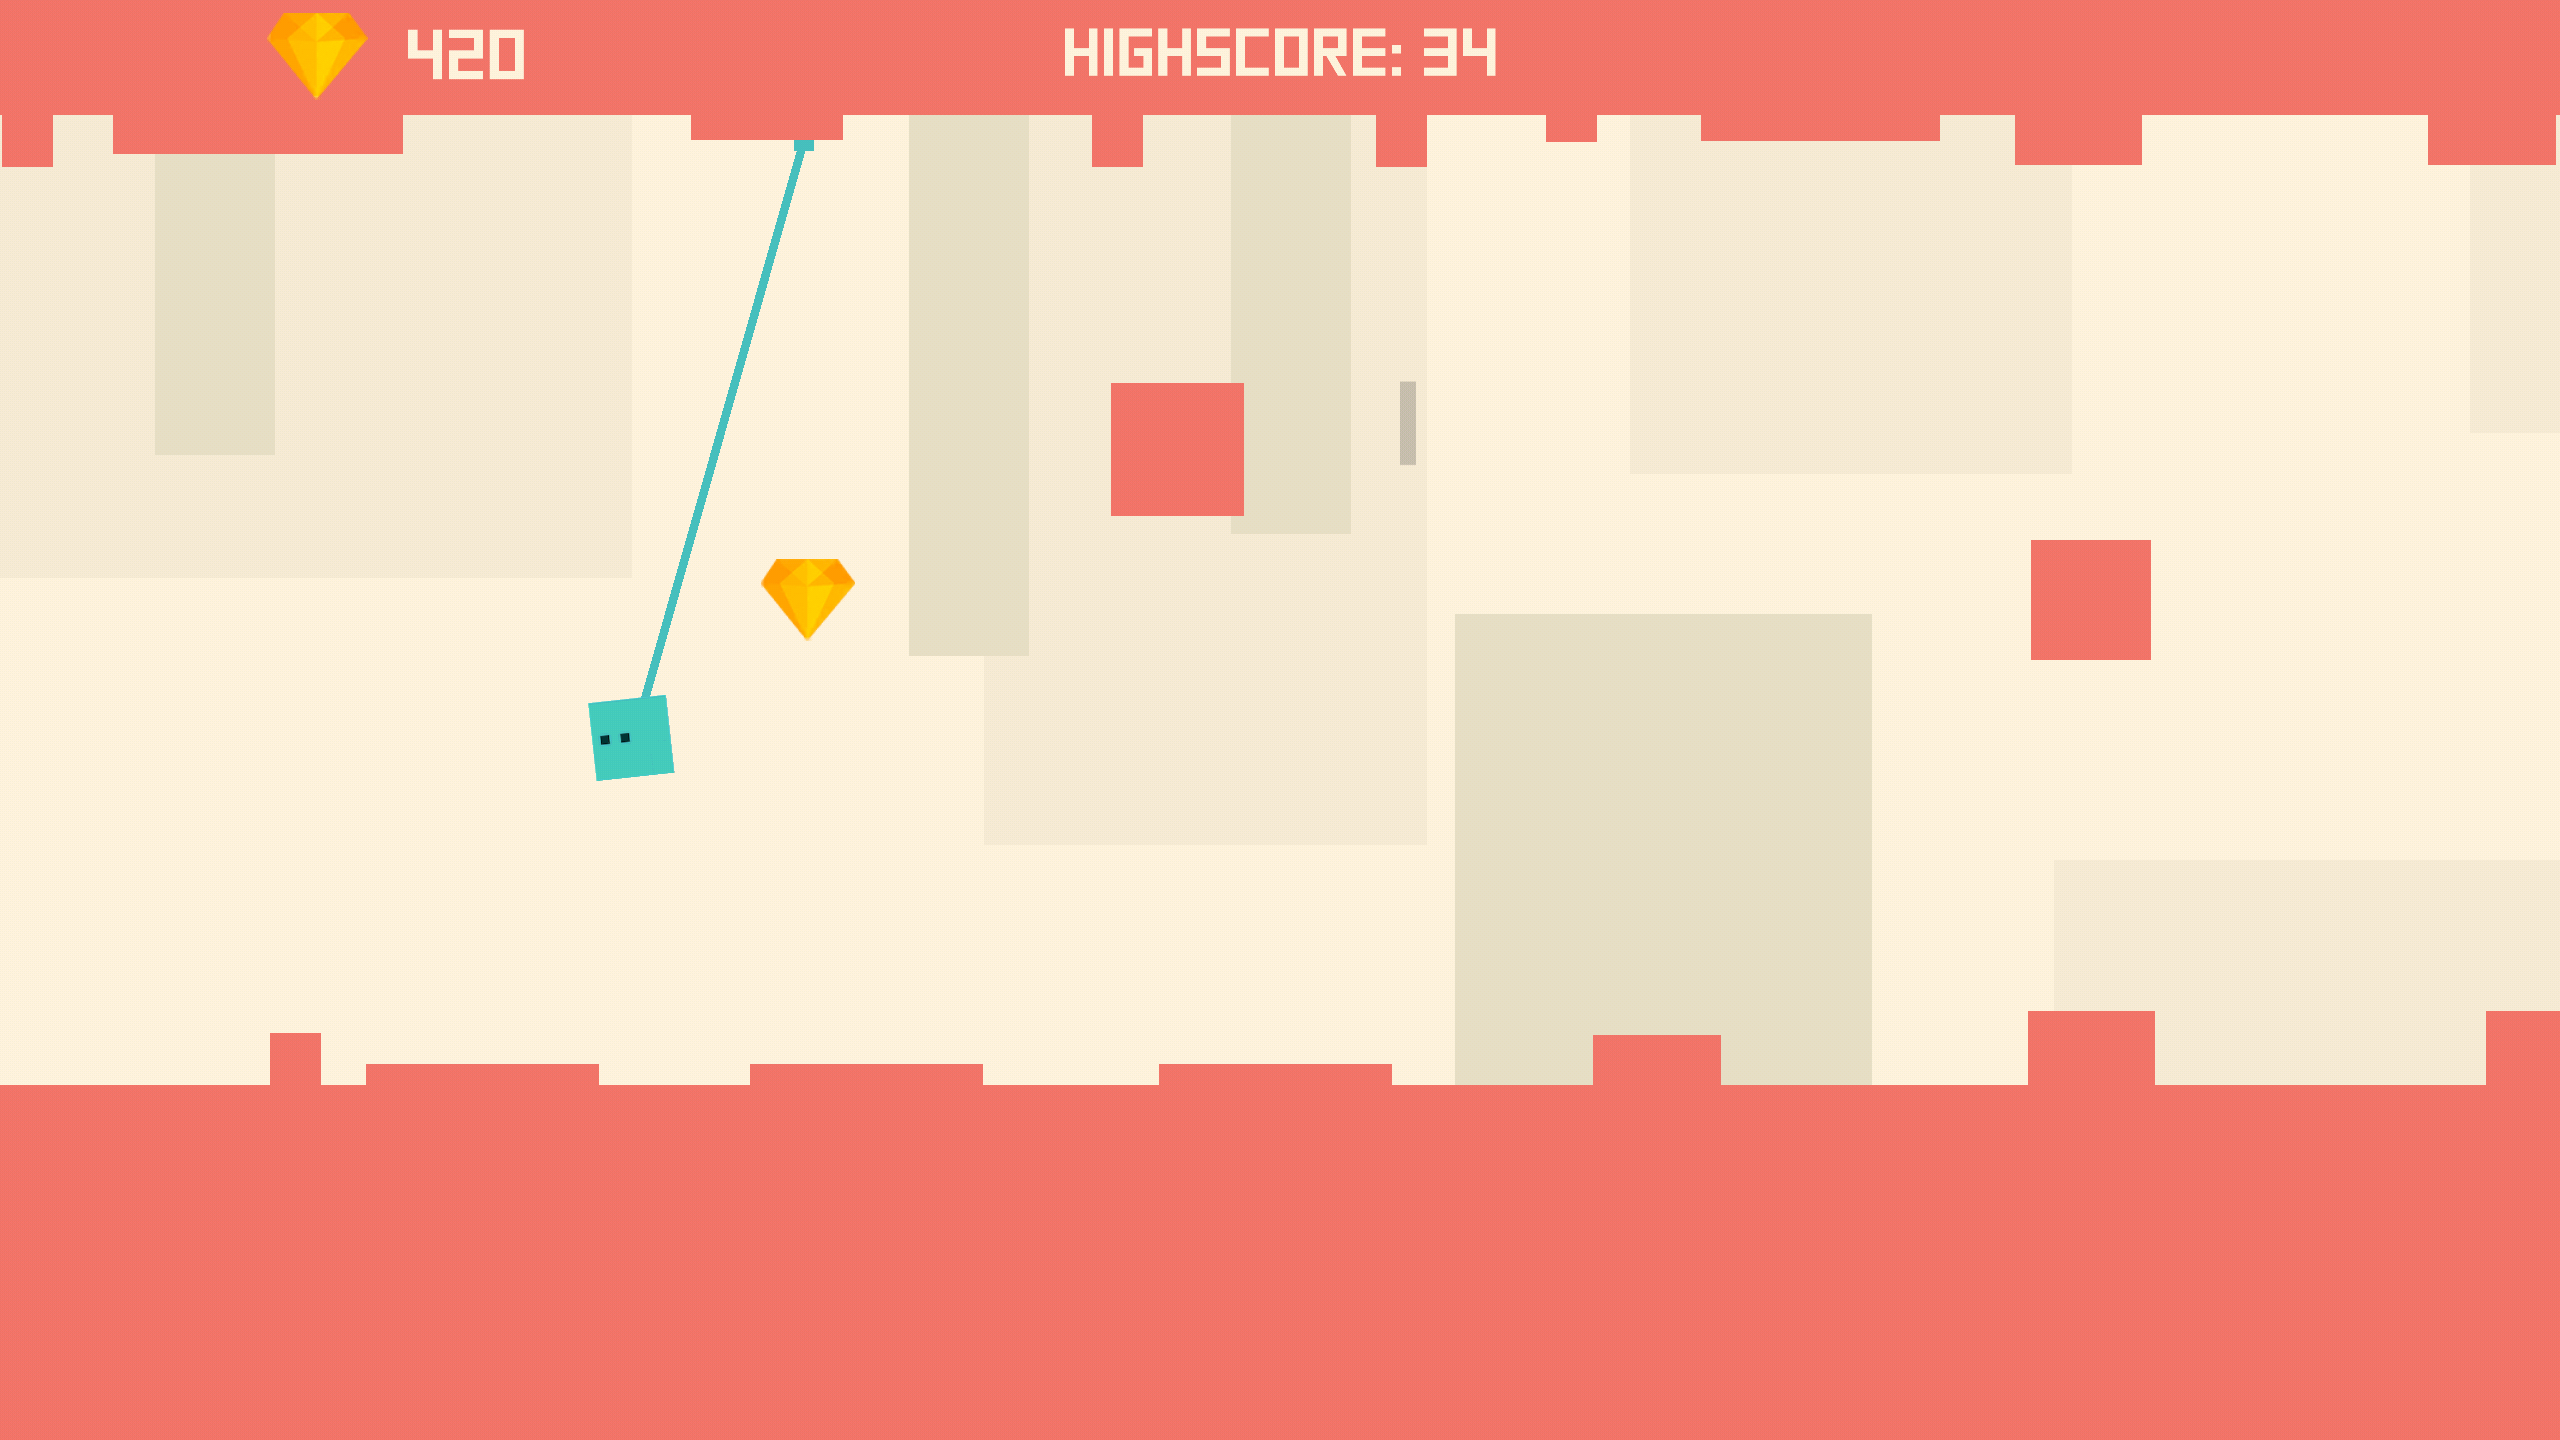
\includegraphics[width=\linewidth]{spider.png}
    \caption{Spider Square screenshot}
    \label{fig:spider}
\end{figure}


As shown in Figure \ref{fig:spider}, the blue square is the player's character,
with the red floor, ceiling, and blocks represent obstacles that destroy the
character and cause the game to end. The player moves the square through the
level by tapping anywhere on the screen to cast the ``web'', a blue line drawn
from the square to the ceiling that pulls the square to the right and upward,
progressing through the level. The blue square's horizontal position never
changes, the level moves around the player. Moving obstacles and narrower
passages appear as the player progresses in the game.

The goal for this project was to create a standalone robotic controller for a
mobile phone capable of capturing the phone's screen and driving the input to
the game in such a way that the player progressed as far as possible without
colliding with the stage.

\section{Methodology}

\section{Results}

\section{Conclusion}

\section{References}


\end{document}
